
%\documentclass[a4paper, twoside]{article}

%%\usepackage{icgst}
%\documentclass[12pt,times,a4paper]{article}%[10pt]{article}
%% Use the option review to obtain double line spacing
 \documentclass[preprint,1p,times,review]{elsarticle}

%% Use the options 1p,twocolumn; 3p; 3p,twocolumn; 5p; or 5p,twocolumn
%% for a journal layout:
%% \documentclass[final,1p,times]{elsarticle}
%% \documentclass[final,1p,times,twocolumn]{elsarticle}
%% \documentclass[final,3p,times]{elsarticle}
%\usepackage{spconf}
\usepackage{amsmath}
%\usepackage{named}
%\usepackage{hyperref}
%\usepackage[dvips,pdftex]{hyperref}
%\usepackage{subfigure}
\usepackage{array}
\usepackage{amssymb}
%\usepackage{epsfig}
%\usepackage{epstopdf}
%\usepackage{xltxtra}
\usepackage{graphicx}
\usepackage{subfigure}
\usepackage{sectsty}
%\sectionfont{\normalsize  }
%\subsectionfont{ \normalsize\it \textbf }
%\subsubsectionfont{\normalsize \it \textbf }
%\paragraphfont{\large\it}
%\subparagraphfont{\normalsize\it}

%% The lineno packages adds line numbers. Start line numbering with
%% \begin{linenumbers}, end it with \end{linenumbers}. Or switch it on
%% for the whole article with \linenumbers after \end{frontmatter}.
%% \usepackage{lineno}

%% natbib.sty is loaded by default. However, natbib options can be
%% provided with \biboptions{...} command. Following options are
%% valid:

%%   round  -  round parentheses are used (default)
%%   square -  square brackets are used   [option]
%%   curly  -  curly braces are used      {option}
%%   angle  -  angle brackets are used    <option>
%%   semicolon  -  multiple citations separated by semi-colon
%%   colon  - same as semicolon, an earlier confusion
%%   comma  -  separated by comma
%%   numbers-  selects numerical citations
%%   super  -  numerical citations as superscripts
%%   sort   -  sorts multiple citations according to order in ref. list
%%   sort&compress   -  like sort, but also compresses numerical citations
%%   compress - compresses without sorting
%%
%% \biboptions{comma,round}

% \biboptions{}
% \setlength\hoffset{0in}
% % \setlength\topmargin{0in}
% % \setlength\headheight{0in}
% % \setlength\headsep{-0.5in}
% % \setlength\textheight{10.0in}
%  \setlength\textwidth{7in}
%  \setlength\oddsidemargin{-0.5in}
%  \setlength\evensidemargin{-0.5in}
% % \setlength\parindent{0.25in}
% % \setlength\parskip{0.25in}
% \linespread{1.5}
\begin{abstract}

%This study
%%%This study

Sketches and drawings are widely used as a simple method of expressing thought and designs. The goal of this paper is developing a sketch recognition system that facilitates using sketches in computer systems. The system uses Particle Swarm Algorithms to optimally segment the strokes the user draws into meaningful geometric primitives.  These geometric primitives are grouped to formulate symbols which are further identified using a Support Vector Machines (SVM) classifier. A comparision is presented between using Traditional Particle Swarm Optimization and the Enhanced Particle Swarm Optimization (EPSO) which is based on the perturbation of the particle velocity. Two different segmentation algorithms were evaluated and results show that both algorithms improve the final recognition results. Experiments were conducted on three different dataset, simple presentation (Hs-DS), Electrical Design (EL-DS) and Logic Design (LD-DS) symbols. Results show that the effectiveness of the proposed system on various dataset especially on datasets with low shape diversity as in Logic Design dataset (LD-DS). Results also show that using an Enhancment on the Tradiontal Swarm algorithm improves recognition rate.

\end{abstract}
\begin{document}


%\begin{frontmatter}
%% Title, authors and addresses

%% use the tnoteref command within \title for footnotes;
%% use the tnotetext command for the associated footnote;
%% use the fnref command within \author or \address for footnotes;
%% use the fntext command for the associated footnote;
%% use the corref command within \author for corresponding author footnotes;
%% use the cortext command for the associated footnote;
%% use the ead command for the email address,
%% and the form \ead[url] for the home page:
%%
%% \title{Title\tnoteref{label1}}
%% \tnotetext[label1]{}
%% \author{Name\corref{cor1}\fnref{label2}}
%% \ead{email address}
%% \ead[url]{home page}
%% \fntext[label2]{}
%% \cortext[cor1]{}
%% \address{Address\fnref{label3}}
%% \fntext[label3]{}


%% use optional labels to link authors explicitly to addresses:
%% \author[label1,label2]{<author name>}
%% \address[label1]{<address>}
%% \address[label2]{<address>}


\title{Sketch Recognition using Enhanced Particle Swarm Optimization}

% \twocolumn[
% \scalebox{1.00}{
\includegraphics[width=1.00\textwidth]{aimlhead}}
% \title{Sketch Recognition using Enhanced Particle Swarm Optimization}
% \vspace{0.1in}
% \author{}
% \begin{center}
% Maha El Meseery\footnote{Corresponding Author }, Mahmoud Fakhr El Din, Tarek
%abouldahab\\
% \textit{Electronic Research Institute,} Cairo, Egypt,\\
% \textit{ Cairo Metro Company, Ministry of transport }Cairo, Egypt\\
% {melmeseery@eri.sci.eg, mafakhr@mcit.gov.eg,  heshoaboda@hotmail.com},\\
% %\texttt{http://www.faculty.university.edu.any}
% \end{center}
% \vspace{0.25in}
% ]

% \twoauthors
%
%  {Maha El Meseery, Mahmoud Fakhr El Din}
% 	{Signals Processing Group \\ Computers and Systems Department \\
%   Electronic Research Institute\\Cairo, Egypt\\
% 	melmeseery@eri.sci.eg, mafakhr@mcit.gov.eg}
% 	 {Tarek abouldahab\sthanks{Corresponding Author}} {Cairo Metro Company
%\\
%   Ministry of transport \\Cairo, Egypt\\ heshoaboda@hotmail.com}

% \author[Eri]{Maha El Meseery \corref{cor1} }%,
% \ead{melmeseery@eri.sci.eg}
% \author[Eri]{Mahmoud Fakhr El Din}
% \ead{ mafakhr@mcit.gov.eg}
% \author[metro]{Tarek abouldahab}
% \ead{heshoaboda@hotmail.com}
%
% \address[Eri]{Signals Processing Group, Computers and Systems Department,
%   Electronic Research Institute,Cairo, Egypt.}
%   \address[metro]{Cairo Metro Company, Ministry of transport ,Cairo, Egypt.}
% \cortext[cor1]{ Corresponding author}

\author{
\small{
Maha El Meseery \footnote{Corresponding Author} \textsuperscript{a}, Mahmoud
Fakhr El Din \textsuperscript{a}, Tarek abouldahab \textsuperscript{b}}\\
 \textsuperscript{a} \small{Signals Processing Group, Computers and Systems
Department,}\\ \small{ Electronic Research Institute, Cairo, Egypt.}\\
  \small {\textsuperscript{b}Cairo Metro Company ,
   Ministry of transport , Cairo, Egypt.}\\
   \small{melemseery@eri.sci.eg,  mafakhr@mcit.gov.eg, heshoaboda@hotmail.com
   }
}
\date{}
% {\sthanks{Corresponding Author},}
% 	{Signals Processing Group \\ Computers and Systems Department \\
%   Electronic Research Institute\\Cairo, Egypt\\
% 	melmeseery@eri.sci.eg, mafakhr@mcit.gov.eg}
%   {Tarek abouldahab} {Cairo Metro Company \\
%   Ministry of transport \\Cairo, Egypt\\ heshoaboda@hotmail.com}
%  {Maha El Meseery \sthanks{Corresponding Author}, Mahmoud Fakhr El Din}
% 	{Signals Processing Group \\ Computers and Systems Department \\
%   Electronic Research Institute\\Cairo, Egypt\\
% 	melmeseery@eri.sci.eg, mafakhr@mcit.gov.eg}
% 	 {Tarek abouldahab\sthanks{Corresponding Author}} {Cairo Metro Company
%\\
%   Ministry of transport \\Cairo, Egypt\\ heshoaboda@hotmail.com}

\maketitle
%  \begin{abstract}
%
% %This study
% %%%This study
%
% Sketches and drawings are widely used as a simple method of expressing thought and designs. The goal of this paper is developing a sketch recognition system that facilitates using sketches in computer systems. The system uses Particle Swarm Optimization (PSO) algorithm to optimally segment the strokes the user draws into meaningful geometric primitives.  These geometric primitives are grouped to formulate symbols which are further identified using a Support Vector Machines (SVM) classifier. Two different segmentation algorithms were evaluated and results show that both algorithms improve the final recognition results. Experiments were conducted on three different dataset, simple presentation (Hs-DS), Electrical Design (EL-DS) and Logic Design (LD-DS) symbols. Results show that the effectiveness of the proposed system on various dataset especially on datasets with low shape diversity as in Logic Design dataset (LD-DS).
%
%
%  \textsl{Sketches and drawings are widely used as a simple method of expressing
% thought and designs. The goal of this paper is to improve our sketch recognition
% system by using an enhanced particle swarm optimization algorithm. The Enhanced
% Particle Swarm Optimization (EPSO) is based on the perturbation of the particle
% velocity is used to optimally segment the strokes the user draws into meaningful
% geometric primitives. These geometric primitives are grouped to formulate
% symbols which are further identified using a Support Vector Machines (SVM)
% classifier. Experiments were conducted on the benchmark dataset of simple
% presentation (Hs-DS) symbols. Results show that the enhanced particle swarm
% optimization improves the final recognition accuracy.}
% \end{abstract}

% \begin{keyword}
% %% keywords here, in the form: keyword \sep keyword
%
% %% MSC codes here, in the form: \MSC code \sep code
% Sketch Recognition, Particle Swarm Optimization
% %% or \MSC[2008] code \sep code (2000 is the default)
%
% \end{keyword}
%\end{frontmatter}
\textit{\textbf{Keywords:} Sketch Recognition, Particle Swarm Optimization.}
%\pagenumbering{arabic}
 \section{Introduction}

 The field of symbol recognition has gained interest in the last few years. Scientists generally and engineers specifically express thoughts and designs using sketches. Engineers use sketches to exchange designs as a natural method of communication rather than writing or speaking. Design engineers need a powerful computer based system with symbol recognition to help them design, manipulate and store sketches more effectively than using only papers. Increasing the interaction between computers and users in sketch and CAD systems has been the reason for the emerging of a few advanced sketch recognition systems. Sketch recognition is the process of identifying user strokes into meaningful symbols that can be further used. 

 Sketch recognition is divided into three main steps preprocessing, segmentation and symbol recognition. The preprocessing phase captures user input stroke points and collects basic information about the stroke then proceeds to remove noise and compute basic statistical and geometrical information. In segmentation phase, the strokes are divided into a set of simple geometrical primitives or segments. In the third phase, sketch recognition, strokes and segments are clustered to formulate symbols that can be recognized by a classifier system.



In PR based methods, systems compute properties that describe symbols then use a classification method to recognize symbols. The properties used can either be based on gesture properties, global shape properties or image based properties. Gesture properties are set of features that represent how the user draws a symbol not how it looks like (e.g., identify a rectangle when a user draws a L corner). In gesture properties approach, systems identify symbols by using gesture properties of some of its underlying strokes. A system that uses gestures properties assumes that users draws symbols in specific order and style \cite{gestureexample12,aideddesgin22}. In global shape properties approach, systems investigate general shape properties and its underlying strokes. Using shape properties (e.g., ratio of the area of convex hull to the area of shape) relaxes the assumption and the role of each stroke in the symbol but it does not truly represent the appearance or fine details of the symbol \cite{DiagramOfflineConvexHull,Cali63}. Unlike shape properties based methods, image based methods disregard individual strokes and focus on the overall appearance of shapes. These system convert the shapes into image and extracted image based features (e.g. local gradient feature)\cite{Oltmans07,imagetrainable48}. In \cite{imagetrainable48}, they used four different distance measures to match user symbol with the prototype database. The prototype of a shape is represented as an image of the symbol that is normalized and scaled.  However, the problem is that the shape prototype must represent all transformation and variation the input shape can have.   %Image based methods are used in \cite{Oltmans07,imagetrainable48} where they computed a code book of 1000 features to recognize symbols. 

 Methods based on gesture and global shape properties produce systems that are dependent on assumptions about how strokes can be grouped. These systems assume that users will finish drawing a shape before moving to the next one \cite{Cali63,geometrydomain49}. This assumption allows the system to temporally group strokes and then recognizes them based on their strokes or global shape properties. Alvarado \cite{AlvaradoDigital} argued that this assumption does not hold in natural sketches.


In this paper, we choose to implement a hybrid method that includes shape property, gesture and hierarchical information. Our method attempts to avoid many of the problems faced by approaches based on individual gestures or global shape properties while trying to gain the additional information that the stroke based system uses. Firstly, the system uses particle swarm optimization (PSO) to optimally segment user's strokes. Users can draw symbols using any number of strokes in any order they like. The system segments each stroke using two different PSO algorithms. The first segmentation algorithm is based on dividing the digital curve into polygons\cite{PolygonApproximationPSO}. Our algorithm enhances its performance by adding curvature and other local information during segmenting strokes to achieve better results. To handle complex strokes, our system uses a second segmentation PSO algorithm that segment strokes into a set of lines and circular arcs. The two segmentation algorithms can either by used individually or in parallel then chosing the segmentation that gives the minimum error. After segmentation, a feature vector composed of different statistical, geometrical and composite features is deduced. The final classification step uses a SVM classifier to classify symbols into one of the previously trained classes based on the features vector computed\cite{mypaper}.
  
  
  In addition to the system mentioned above, an Enhnaced Swarm algorithm is compared to the Traditional Particle swarm algorithm\cite{stockPaper}. The Enhanced swarm algorithm is based on chaning the particle velocity by replacing it with the weighted differance between the particle and another random in the space. This random relacing is only used when the new velociy and location is better then the current particle values. The procedure introude new expolration factor the swarm system which helps in reaching the solution faster and more obtimially.






% %This paper modifies the sketch recognition system presented in \cite{mypaper},
% to use enhanced particle swarm algorithm (EPSO) to optimally segment user's
% strokes. As in the Original system the users can draw symbols using any number
% of strokes in any order they like. The system segments each stroke using two
% different EPSO algorithms. Segmentation is based on dividing the digital curve
% into polygon\cite{PolygonApproximationPSO}. To handle complex strokes, our
% system uses a second segmentation EPSO algorithm to segment strokes into a set
% of lines and circular arcs. After segmentation, a symbol features vector
% composed of different statistical, geometrical and spatial features is deduced.
% The final classification step, SVM classifier uses the computed feature vector
% to classify the segments into one of the previously trained classes.

The remaining of the paper is as following; Section
\ref{sec:ParticleSwarmAlgorithm} describes the Basic particle swarm algorithm in
details.  Enhanced Particle Swarm Algorithm is described in Section
\ref{sec:EnhancedSwarmAlgorithm}. Section \ref{Sysdisc} provide details on
preprocessing, segmentation and recognition process. Section
\ref{sec:Experiments} describes the experiments that were preformed. We conclude
in Section \ref{ConclusionandFutureWork}.


\section{Basic Particle Swarm Optimization}
\label{sec:ParticleSwarmAlgorithm}
 
 Particle Swarm Algorithm\cite{PSOFirst}is a population based stochastic search where each solution is simulated as a  particle that flies around in a multidimensional search space. A fitness function is used to evaluate the goodness of each particle in solution space. But unlike evolutionarily algorithm the new population is the PSO is influenced by the social cooperation of the particle rather than survival to the fittest. Each particle saves a history of the best location in the swarm and its own best location.  At the end each iteration, the particles moves to a new location based on the global best location and it own history of best location. This use of previous particle locations gives PSO advantage over Evolutionary algorithms where no similar information is used.

 The \textit{Basic Particle Swarm Algorithm (PSO)} represents each solution with a $N$ dimension particle from the solution space \cite{PSOFirst}. Each particle moves with a direction and velocity $v_{ij}$ based on equations \ref{eq:Swarm1} \& \ref{eq:Swarm}.


\begin{equation}
%\[
p_{ij}=p_{ij}+v_{ij},
%\
\label{eq:Swarm1}
\end{equation}

where $p_{ij}$ represent the $j$th dimension in the $i$th particle and $v_{ij}$ is the velocity of the $j$th dimension in the $i$th particle.

 \begin{equation}
v_{ij}  = v_{ij} \omega + c_1 r_1 (lbest_{ij}  - p_{ij} ) + c_2 r_2 (gbest_{ij}
- p_{ij} ),
\label{eq:Swarm}
\end{equation}
 where $\omega$ is the inertia weight parameter which controls the tradeoff between exploration and exploitation,  $lbest_{ij}$ is the local best particle, $gbest_{ij}$ is the global best particle, $r_1$ \& $r_2$ are random variables and $c_1$ \& $c_2$ are the swarm acceleration parameters.

 After each iteration the global best $g_{best}$ particle and the agent local best particle $l_{best}$are evaluated based on the maximum fitness functions of all particles in the solution space. The solution is found after achieving a specific number of iteration or after an error threshold is achieved.

\section{Enhanced Particle Swarm}
\label{sec:EnhancedSwarmAlgorithm} 

In the above basic PSO, the velocity update is based on three terms an inertia term, local cognitive ($l_{best}$) term and global cognitive ($g_{best}$)term. The particle local cognitive term is associated with the particle own history without consideration of other swarm particles locations and histories which leads to a lake of diversity and sub optimum solutions. Therefore, we are trying to add more social influence in the particle movement by using the weighted difference of the position vectors of any other two distinct particles randomly chosen from the swarm to modify the local cognitive term. The modified term adds social behavior of other particle and keeps diversity while searching for the global optimum. The new social cognitive term of the particle is shifted to the new location only if it yields a fitness value better than obtained using the standard PSO\cite{stockPaper}.

This modification is done as follows:-
  \begin{enumerate} \item For each particle $p_{i}$ in the swarm two other distinct particles, $p_L$ and $p_M$ are selected randomly where $i\neq L\neq M$. The difference between their positional coordinates $p_{d}$ is taken as a difference vector in equation
\ref{eqmod}.
 \begin{equation}
 \label{eqmod}
 p_{dj}= p_{Lj}-p_{Mj}
 \end{equation}
where $p_{dj}$ represent the $j$th dimension in the difference vector and
$p_{Lj}$ represent the $j$th dimension in the $L$th particle.

Then the associated velocity vector of particle $p_{i}$ is updated according to this difference vector as in equation \ref{eq:mod1}. In essence the local cognitive term of the velocity update formula in \ref{eq:Swarm} is replaced with the vector differential operator $p_d$ to produce some additional exploration capability.
 \begin{equation}
 v^{T}_{ij}  = v_{ij} \omega + c_1 r_1 (p_{dj}) + c_2 r_2 (gbest_{ij}  - p_{ij}
),
 \label{eq:mod1}
 \end{equation}
\item The new trial position $p^{T}_{ij}$ is created by adding the updated
velocity $v^{T}_{ij}$ in Eq. \ref{eq:mod1}.
  \begin{equation}
 \label{eq:mod2}
p^{T}_{ij}=p_{ij}+ v^{T}_{ij} ,
 \end{equation}
\item The new position $p^{T}_{ij}$ is used to generate the new trial objective fitness function value $fitness(p^{T})$. The fitness value is calculated based on this new trial position vector and the particle is shifted to this trial position if the trial objective function is better than the original objective function associated with standard PSO. Thus the target particle is relocated using the following equation (Eq. \ref{eq:objective})
  \begin{equation}
 \label{eq:objective}
p^{new}_{ij}\Leftarrow
\{
\begin{array}{c}
 p^{T}_{ij} \quad \quad if\quad fitness(p^{T})> fitness(p^{old})  \\
 p_{ij} \quad \quad Otherwise\quad
\end{array}\}
 \end{equation}
 where $fitness(p^{T})$ is the objective fitness value of the new trail position
$ p^{T}$ and  $fitness(p^{old})$is the objective fitness value of the new basic
position $ p{i}$ computed by equation \ref{eq:Swarm1}.
   \end{enumerate}

\section{System Discribtion  }\label{Sysdisc}
%\label{sec:application}
%The modified swarm algorithm is used to improve the performance of the sketch recognition system in \cite{mypaper}.
 The sketch recognitions system is divided into three main steps 1) preprocessing, 2) segmentation and 3) Recognition. Figure \ref{fig:flowChart} shows the block diagram of the system; the first process is collecting stroke points then computing the curvature and possible dominant points.  The following section provides a detailed description of each step. The main block of the system remains the same but there are some modifications in the segmentation algorithm to improve its efficiency. This study compares between using Traditional PSO and an Enhanced Particle swarm algorithm. Other modifications are explained in the details in the next sections.
%  \begin{figure}
% 	\centering
% 		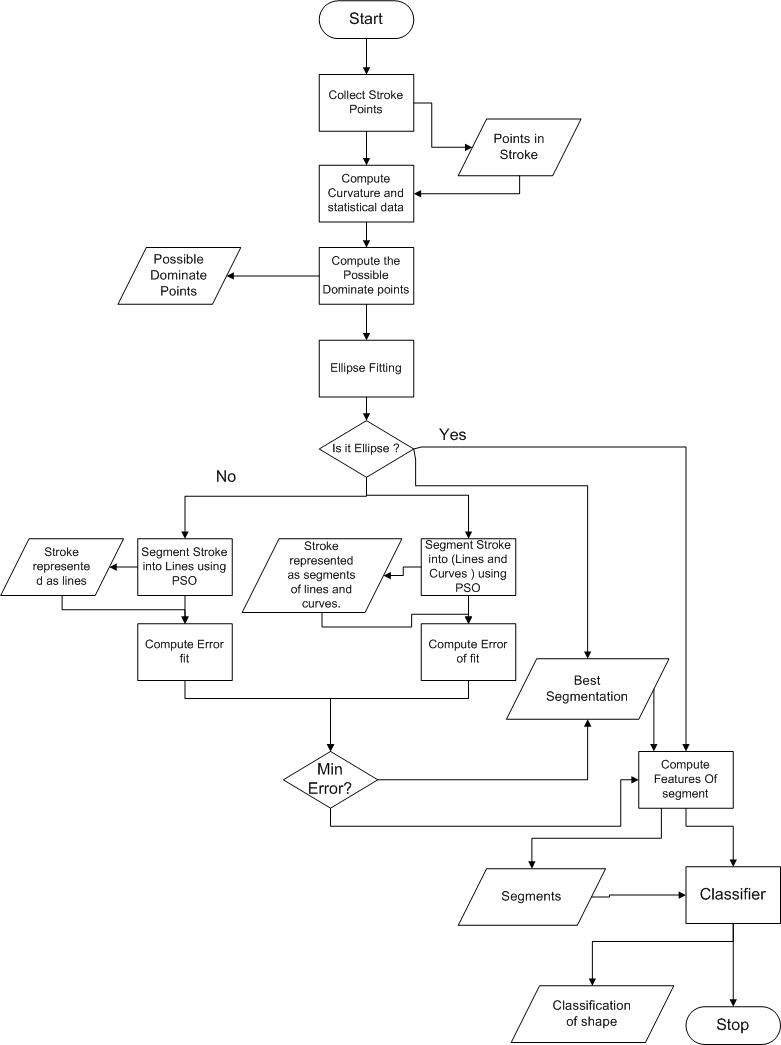
\includegraphics[width=3.5in,height=6in]{FlowChart.jpg}
% 	\caption{System flow chart} The chart shows the flow of process and data processed thought the system.
% 	\label{fig:flowChart}
% \end{figure}

 \begin{figure}
	\centering
		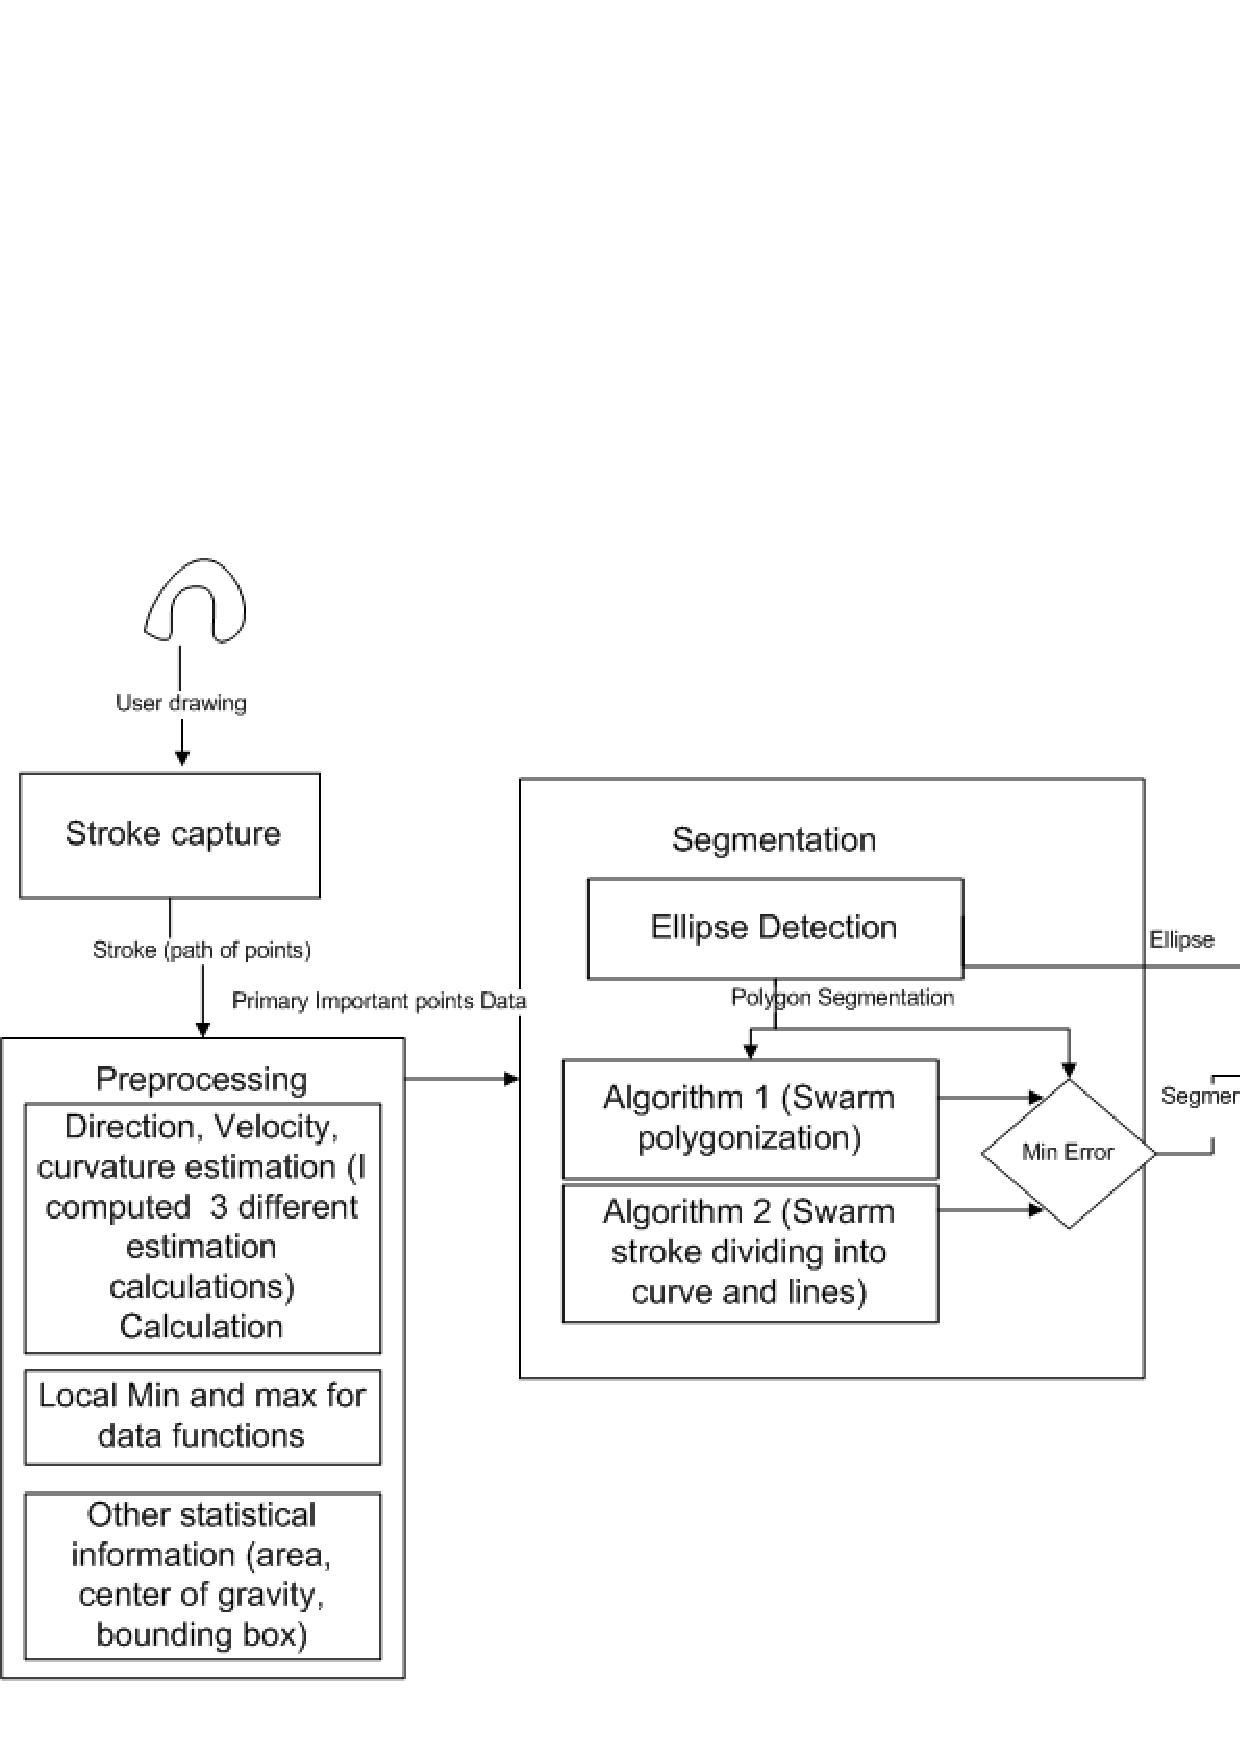
\includegraphics[scale=0.5]{images/Blockdiagram.png}
	\caption{System Block Diagram} The chart shows the system block diagram.
	\label{fig:flowChart}
\end{figure}


\subsection{Preprocessing}
\label{Prepross}
  Speed and time difference information were widely used in sketch recognition systems \cite{earlyprocess}. Figure \ref{fig:orignalStroke} shows an example of an input stroke drawn by users.  Figure \ref{fig:speed2Distance} shows the graph of time difference and the speed for the stroke in Figure \ref{fig:orignalStroke}. It was noted that time difference provides more distinct maxima than the speed information. Agar et al. \cite{polygonfeedback31} mentions that the pointing device (e.g., mouse) sampling rate is the reason for this phenomenon. The points are sampled at regular time intervals as long as the pointing device is moving. Therefore, there are no new detected points when the pointing device is stationary. This leads to a nearly constant time difference between samples while the pen is moving and large difference while the pen is stationary (Figure \ref{fig:timediff}). Contrary to time difference information, the speed information has a lot of noise in the data because usually  users draw with variant speeds (Figure \ref{fig:speed2Distance}).  %Similarly, direction
%information is used as it provides better distinctive maxima for the corners
%than the curvature information \cite{meanshift10}.% Figure \ref{fig:curvatures}
%shows the direction and curvature graphs for the stroke drawn in Figure
\ref{fig:orignalStroke}

 \begin{figure}[h]
	\centering
		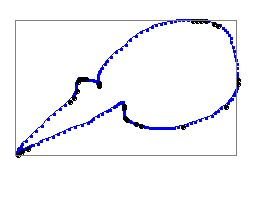
\includegraphics[scale=0.5]{images/stroke3.jpg}
	\caption{Input Stroke} Example of an input stroke to the system.
	\label{fig:orignalStroke}
\end{figure}

 \begin{figure}
	\centering
			\subfigure[Speed versus Displacement Graph]{
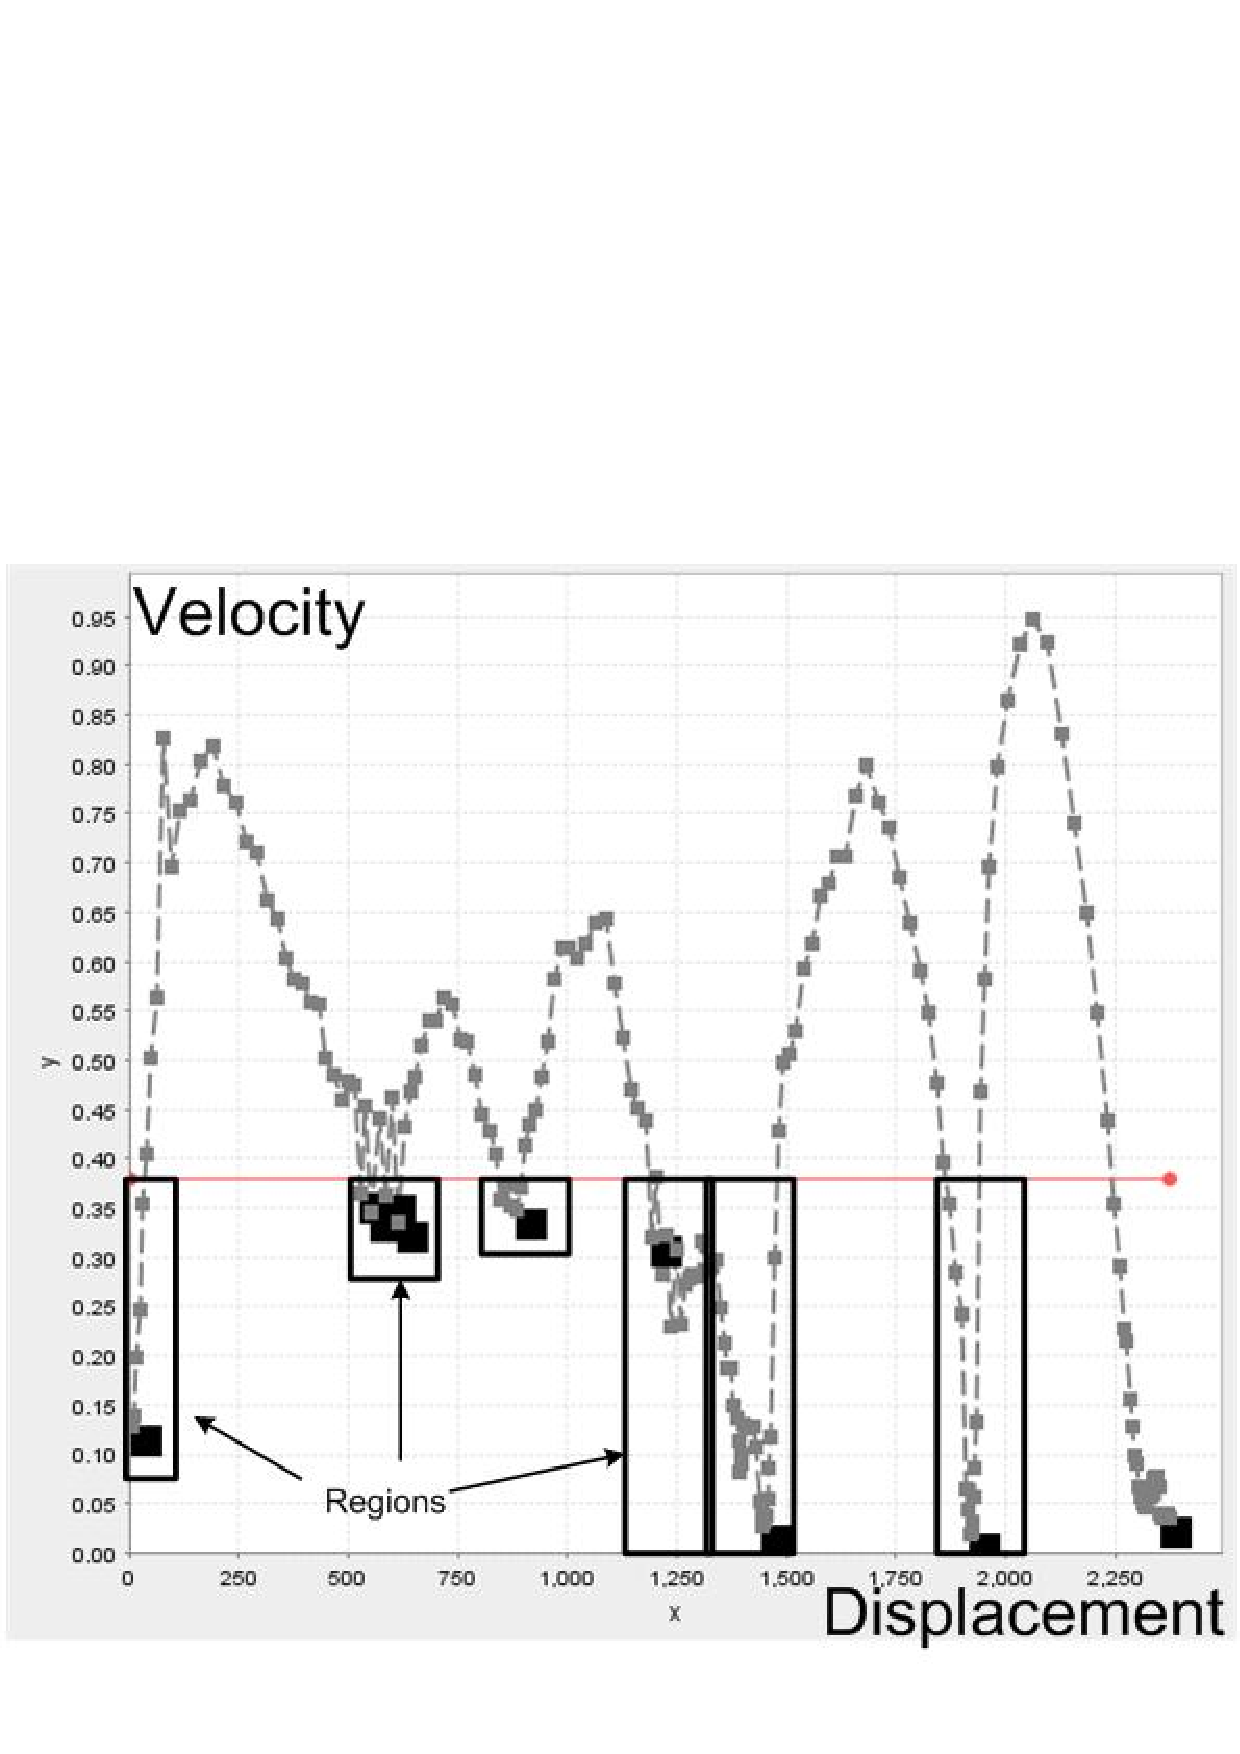
\includegraphics[scale=0.4]{images/vel3.jpg}}
			\hfill
			\subfigure[ Time Difference  versus Displacement
Graph]{\label{fig:timediff}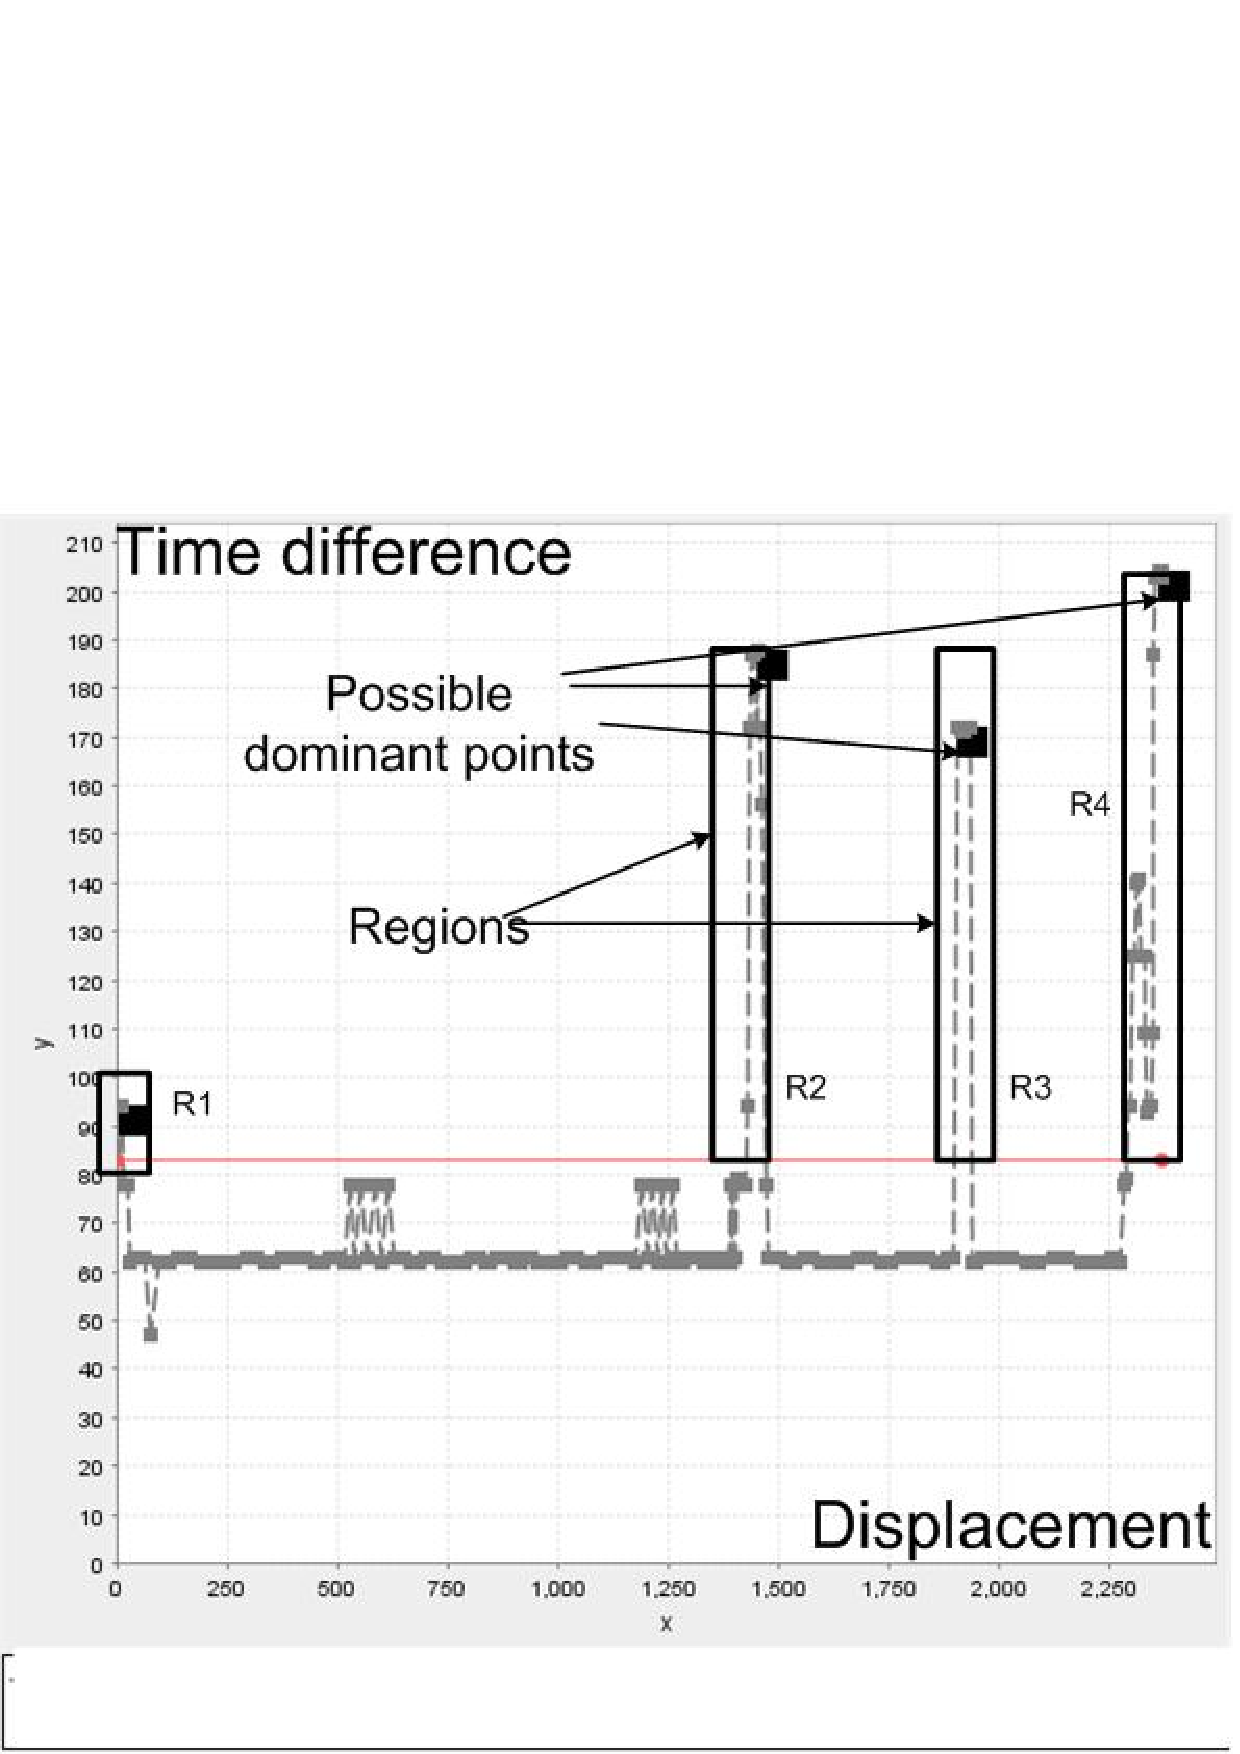
\includegraphics[scale=0.4]{images/td3.jpg}}
	\caption{Speed and Time Difference Graphs}  a) speed graph has lot of
noise in the data with respect to b) time difference.   The black points denote
the location of the possible dominant points $P_{pd}$. Black rectangles
represent regions $R_i$ that in a) Are lower than the threshold. b) Are above
the threshold.
	\label{fig:speed2Distance}
\end{figure}

Dominant points are characterized by low speed values, high curvature and direction values. However, the dominant points from the curvature information may not be the same points as the dominant points extracted from the speed information. Hence, we compute time difference, direction, speed and curvature of each point along a stroke to ensure that no dominant point is overlooked in this phase. The speed is calculated as $v=\Delta s/\Delta t$ where $t$ is the time difference between two points and $s$ is the length between them. The direction $d$ calculated as the angle between vectors $\overrightarrow {P_{i - 1} P_i }$ and the $x-axis$ and the curvature is considered as the change in direction $d$ with respect to length $s$ i.e. $c= \Delta d/\Delta s$.

After the system computes the speed, time difference and curvature information, it proceeds to extracts the points that have low velocity and high curvature. However, using simple differentiation to detect local extreme points results in false points due to the non smooth curves. Hence, our system adopts a process presented by \cite{earlyprocess}, where the mean of each of the four calculated information is calculated. This mean is taken as the threshold \textit{th} which is used to separate the curve into regions ($R_i$) (Figure\ref{fig:timediff}); each region $R_i$ is defined as a range of points, where the curve values are either above or below the threshold \textit{th}. Those regions are further processed to find the maximum point $Max(R_i)$ of each region $R_i$. The stroke points $p_i(x,y)$ that correspond to those maximum values are labeled as \textit{possible dominant points} $P_{pd}$. The system repeats this process for curvature, time difference and speed information. All the points labeled as possible dominant points $P_{pd}$ are saved into a single array. Figure \ref{fig:ppd999} shows the particles labeled as Possible dominate point $P_{pd}$ in the preprocessing phase. It is clear that some of the $P_{pd}$ points are redundant as specified in the preprocessing stage. % (as shown are redundant)
\begin{figure}
	\centering
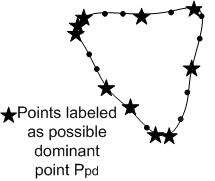
\includegraphics[scale=0.7]{images/ppd.jpg}
	\caption{Possible Dominante Points} An illustration of stroke points and
the expected \textit{possible dominant points} $P_{pd}$.
	%\label{fig:ppd}
	\label{fig:ppd999}
\end{figure}

 
 




\subsection{Segmentation}
\label{seg} 
In the segmentation stage the input stroke is divided into a set of primitives. As shown in Figure \ref{fig:segblock} first an attempt is made to fit the stroke points into a curve or an ellipse using a minimum square error fitting algorithm \cite{ellipsefit}. The ellipse fitting step helps to prevent the system from over segmenting the stroke into multiple lines or curves if the input stroke is an ellipse. If the stroke proved to be an ellipse arc then the segmentation process ends and the system proceeds to the next step. Otherwise, the stroke is passed to two further segmentation algorithms that divide the stroke to either lines or lines and curves. After two different segmentations are generated, the system chooses the segmentation with the minimum error. The following sections describe in details the ellipse detection algorithm and the two segmentation algorithms used to divide the stroke.

 \begin{figure}
	\centering
		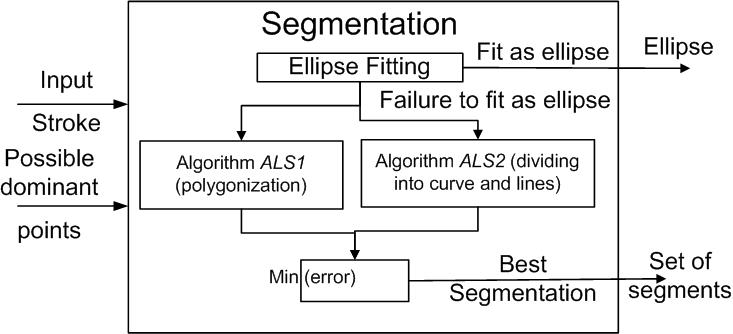
\includegraphics[scale=0.48]{blockSmall.jpg}
	\caption{Segmentation Block}
	\label{fig:segblock}
\end{figure}
\subsection{Ellipse fitting}  This process tries to fit the stroke points into an ellipse arc; it starts with computing the center of the stroke bounding box. The bounding box center point is used as the first estimation of the center of the ellipse. The axes of the ellipse are estimated as the $width/2$ and $height/2$ of the stroke bounding box where $width$ is width and $height$ is height of the bonding box. The least square fitting algorithm \cite{chernov} is used to minimize the fitting error of the ellipse Equation (\ref{eq:circleFit})

\begin{equation}
E = \sum\limits_{i = 0}^N {\frac{{(x_i - x_0 )}}{{a^2 }}^2  + \frac{{(y_i - y_0
)}}{{b^2 }}^2  - 1}
\label{eq:circleFit}
\end{equation}
  where $N$ is number of points in the stroke, $a,b$ are the length of ellipse axes, $x_0$ \& $y_0$ are the coordinates of the center point, $x_i$ \& $y_i$ are the coordinates of point $i$ in the stroke. A list of new values for $x_0$ , $y_0$ ,$a$ and $b$ are generated randomly from the older values with small increments after each loop.  After few iteration, the final fit error of the estimated ellipse is reported. A modification to the system in \cite{mypaper} is trying to add another measure to compute the efficiency of the final estimated ellipse. Equation \ref{eq:circleError} ensures that the drawn percentage of ellipse is considered. This eliminates fitting a line into very large ellipse but leaves small ellipses to be fitted as a partial or full ellipse.

 \begin{equation}
eff= (P_{percent}/E)
\label{eq:circleError}
\end{equation}
 \begin{equation}
P_{percent}  = L_{stroke} /P_{ellipse}
\label{eq:ErrorArea}
\end{equation}
where $E$ is the error computed by Equation(\ref{eq:circleFit}), $L_{stroke}$ total length of stroke and $P_{ellipse} $ is the perimeter of the estimated ellipse. If $eff$ is more than threshold $th_{Ellipse}$\footnote{By trial and error best threshold found was $th_{Ellipse}=0.2$} then the stroke is segmented as an ellipse otherwise the system proceeds to the next step.

\subsection{Non ellipse fitting algorithm}
\label{subsubsec:Discreteparticleswarmalgorithm}
\begin{figure}
	\centering

	 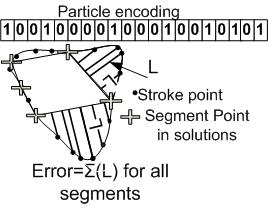
\includegraphics[scale=0.7]{pso1.jpg}
	\caption{DPSO algorithm encoding}
	\label{fig:pso1}
\end{figure}

Two DPSO algorithms are used to generate different segmentations for each stroke the user draws. For each segmentation generated, an error is evaluated. The segmentation with the minimum error value is chosen as the best stroke segmentation (Figure \ref{fig:segblock}). The problem definition is the same in both algorithms but they differ in the method they use to compute fitness and error functions.
\begin{description}
	\item[ Problem definition:] The input stroke $S$  with $N$ points can be
represented by set $S = \left\{ {x_1 ,x_2  \ldots x_N }\right\}$ where $x_i$ is the location of the point $i$. The swarm algorithms consist of $M$ agents which are represented by the set $A = \left\{ {P_i \left| {i = 1,2 \cdots M} \right.} \right\}$ where $P_i$ is a single solution particle from the solution space. Each particle decodes the problem using a binary array with the same length $N$ as the input stroke.

Therefore, the system represents each particle $P_i$ by $P_i = \left\{ {p_{ij}
\left| {j = 1,2 \cdots N} \right.} \right\}$ where $p_{ij}$ has only two values
a)1 ($p_{ij}=1$); means that this point ($j$) is a dominate point, or b)
0($p_{ij}=0$) means this point ($j$) is not a dominate point.
Figure\ref{fig:pso1} shows a particle encoding in the DPSO system.
	\item[Fitness function:] The fitness function and error calculation are
different in each of the two \textit{DPSO} algorithms.
	\end{description}
\subsubsection{\textit{Polygon approximation\textsl{AlgS1}}}
%\\
The approximation error is computed by the equation \ref{eq:ErrorSwarm1}. The
graphical meaning of the error is shown in Figure\ref{fig:pso1}.%\ref{fig:LabelsPSO}.
\begin{equation}
E=\sum\nolimits_{i = 0}^M e ( \widehat{x_ix_{i+1}},\overline{x_i x_{i+1}}) \label{eq:ErrorSwarm1} \end{equation} 
where the arc $\widehat{x_ix_j}$ is defined as the consecutive set of points from point $x_i$ to point $x_{j}$ as in $x_i,x_{i+1} \cdots,x_j$. The line $\overline{x_i x_j} $ as the straight line connecting point $x_i$ to point $x_j$, $M$ is the number of dominant points in this solution as generated by the swarm algorithm. The error $e ( \widehat{x_ix_j},\overline{x_i x_j})$ is computed as the sum of squared perpendicular distance from every point along the arc $\widehat{x_ix_j}$ to the line $\overline{x_i x_j}$. The fitness is computed
using equation %\ref{eq:fitnessSwarm1}
\begin{equation}
\max fitness(p_i ) = \left\{ {\begin{array}{*{20}c}
   { - E/\varepsilon N} & {ifE > \varepsilon ,}  \\
   {D/\sum\limits_{j = 1}^N {p_{ij} } } & {otherwise}  \\ 
   \end{array}} \right. \label{eq:fitnessSwarm1} \end{equation} 
   
   where $N$ is the number of points in the stroke, $D$ is the number of points in the solution that was previously labeled as a possible dominant point ($P_{pd}$), $E$ is the computed error and $\varepsilon$ is the error threshold. It should be noticed that when the error is larger than the threshold $\varepsilon$ the fitness is given a -ve value to lower the fitness value of the solution. Otherwise the system favors the lower number of vertices.

 \subsubsection{\textit{Hybrid Fitting \textsl{AlgS2}}} 
 The algorithm has the same problem formulation but different fitness and error functions are used. An attempt is made to fit each segment into a line or circular arc. The errors of both circle and line fit estimations are computed for each segment $S_i=\widehat{x_ix_j}$. The approximation with the lower error value is chosen as the final approximation of this segment $S_i$\cite{CruveDivisionSwarm}. The sum of the approximation errors of all segments is the total error of the particle.  The total error of the particle is computed by equation %\ref{eq:errorSwarm2}
 \begin{equation}
E=\sum\nolimits_{i = 0}^M e(D_i)
\label{eq:errorSwarm2}
\end{equation}where $M$ is the number of segments in the solution as generated
by the swarm algorithm, $D_i$ is the minimum approximation error of curve and
line approximations $min(d_c,d_l)$ where $d_c$ is the circle approximation error
and $d_l$ is the line approximation error as computed by
\cite{CruveDivisionSwarm}.  The fitness is computed by the equation
%\ref{eq:fitnessSwarm2}
\begin{equation}
\max fitness(P_i ) = \frac{1}{{E \times M^k }}
\label{eq:fitnessSwarm2}
\end{equation} where $E$ is the error and $M$ is the number of segments and $k$
is a parameter tweaked to get minimum number of segments. The larger $k$ is, the
more effect the number of segments will have. For our system, $k$ is selected to
be 0.5\cite{CruveDivisionSwarm}. 

 As a modification to the system in \cite{mypaper}. After each iteration, of the swarm algorithm (\textsl{AlgS1} and \textsl{AlgS2}), each particle is refined using the following procedures:
\begin{enumerate}
	\item For each particle $P_i$ each dominant point $P_{ij}$ is checked to find if it was labeled before as a \textit{possible dominant point} $P_{pd}$ (computed as in section \ref{Prepross}). If it was not labeled the point $P_{ij}$ is moved to the nearest labeled point. This ensures that all of the points generated by the DPSO are possible dominant points $P_{pd}$.
 \item The particles are tested to make sure that the distance between every two successive dominate point is larger than $min_D$, where $min_D$ is 5\% of the total length of the stroke.  Otherwise, one of these points are removed based on the error caused by its removal.
 \item Each two successive segments are test to determine if they can be merged into a single segment. If merging the two segments have the same or smaller the error, the two segments are merged. This step ensures that the final segmentation of the system has minimum number of segments.
\end{enumerate}

\subsection{Recognition}
\label{sec:Recognition} 

After the user draws all strokes of the symbol, the set of un-recognized strokes is grouped together along with their segmentation as input to the feature extraction process. A composite set of features is used to generate a single feature vector. The following list describes each feature in details.
%\begin{description}

\subsubsection{Structural and geometrical Features (FS1)}
  They are features that define the structure of the geometrical symbol such as;
 \begin{itemize}
	 \item \emph{Segments:} The number of segments in the symbol.
	 \item \emph{Strokes:} The number of strokes or partial strokes that
created the symbols.
		\item  \emph{Primitives:} The number of primitives in the
symbol. This feature helps when identifying  symbols with mixed geometric
primitives such as cylinders and callouts.
		\item \emph{Curves:} The number of curves or ellipses in the
symbol.
		\item \emph{Lines:} The number of lines in the symbol.
		\item \emph{Perpendicular}\emph{lines:} The number of
perpendicular lines.
		\item \emph{Parallel}\emph{lines:} The number of parallel lines.
		\item \emph{Intersections:} The number of intersection between
lines and curves.
		\item \emph{T intersections:} The number of T intersections.
		\item \emph{L intersections:} The number of L intersections.
		\item \emph{X intersections:} The number of X intersections.

\end{itemize}
\subsubsection{Rubine Features (FS2)} 
  These features were introduced by Rubine \cite{gestureexample12} for single stroke gestures. Such as length of stroke, cosine of starting angle, smoothness of symbol and some features extracted from the bounding box of the symbol.

\subsubsection{Statistical Features (FS3)}
These features use moments and statistical properties such as;
\begin{itemize}
 \item \emph{Zernike moments:} The zernike moments are orthogonal moments which define the distribution of point in the input space. They are invariant to both reflection and rotation of the input shape \cite{ZerMomentOrthogonal}. %The zernike moment were used in \cite{HeloiseBeautification} t.
\end{itemize}
\subsubsection{Composite Features (FS4)}
 These features are composites of different geometrical and statistical
properties of the symbol.
	\begin{itemize}
\item \emph{Size Ratio:} The ratio between width and height of the symbol.
	\item \emph{Ink density:} The density of points inside its bounding
box\cite{GeometryAndDomain102}.
 	\item \emph{Convex Hull Area:} The area of convex hull with respect to
area of bounding box of symbol.
	\item \emph{Convex Hull Perimeter:} The perimeter of convex hull with
respect to total length of symbol.
		\item \emph{Mean Centroidal radius:} The Mean of the centroidal
radius is the distance from each point in the symbol to the center of gravity.
	\item \emph{Mean Time difference:} The mean of the time difference
between each two successive points in the symbol.
  \end{itemize} 
  After computing the features, the symbol is introduced to the classifier as a feature vector. The system uses Support Vector Machine (SVM) classifier with Linear kernel \cite{libsvm}. An OVO classifier structure (object versus object) is used to handle multi-class problem.% A validation algorithm is used to choose the Kernel variables parameters $c, \gamma$.

%After the user draws all strokes of the symbol, the set of un-recognized
% strokes is grouped together along with their segmentation as input to the feature extraction process. A composite set of features is used to generate a single feature vector. The features used consist of Rubine feature set,  Zernike moments of order 10 \cite{HeloiseBeautification}, ink density as well as some structural and spatial information like number of perpendiculars lines ,number of parallel lines and number of different types of primitives in each symbol. After computing the features the symbol is introduced to the (SVM) classifier. \cite{mypaper}
\section{Experiments}
\label{sec:Experiments}
%The paragraph for the single dataset
% In our Experiments the dataset (Figure
% \ref{fig:HsSet}) was collected by Hse and Newton\cite{HeloiseBeautification}
% (Hs-DS). The data are drawn by 16 users each of them was asked to draw 13 shapes
% from 30 to 50 times.The dataset was divided into training and test sets. Five different splits for the
% training and test data are generated from each dataset. The results displayed
% are the average recognition accuracy of the five splits. The accuracy is
% computed as the number of correctly recognized samples divided by the total 
% number of samples in the test.  

In our experiment we used three different datasets. The first dataset (Figure \ref{fig:HsSet}) was collected by Hse and Newton\cite{HeloiseBeautification} (Hs-DS). The data are drawn by 16 users each of them was asked to draw 13 shapes from 30 to 50 times. Figure \ref{fig:ELsymbolSet} and \ref{fig:LogicsymbolSet} shows the symbols we manually gathered from 7 different users in electrical (EL-DS) and logic design (LD-DS) domain respectively.  Table \ref{tab:datasets} shows a comparison between the three datasets used in our experiments. The datasets were divided into training and test sets. Five different splits for the training and test data are generated from each dataset. The results displayed are the average recognition accuracy of the five splits. The accuracy is computed as the number of correctly recognized samples divided by the total number of samples in the test.


\begin{figure}
\centering

\fbox{ \parbox{5cm}{%
		\includegraphics[scale=0.5]{images/symbolSet.PNG}	}}
		\caption{The Hs-DS Symbol Set} The dataset consist of simple presentation symbols.
		\label{fig:HsSet}
\end{figure}
\begin{table}
\begin{center}
\scalebox{0.8}{
 \begin{tabular}{|p{3cm}|p{1.5cm}|p{1.5cm}|p{1.5cm}|}
 \hline
 & Hs-DS &  EL-DS & LD-DS \\ \hline
No of samples  &  7791 & 2764 & 1859 \\ \hline
No of categories  & 13 & 15 & 8 \\ \hline
Avg. Samples per Category& 600 & 184 & 232 \\\hline
No of users  & 16 & 7 & 7 \\  \hline
Balanced & Yes&No & No \\ \hline
Splits  & 5 random splits  & 5 random splits  & 5 random splits  \\ \hline
Examples & Figure \ref{fig:HsSet}  & Figure \ref{fig:ELsymbolSet}  & Figure \ref{fig:LogicsymbolSet}   \\ \hline
\end{tabular}
}
\caption[Datasets Comparisons]{Table compares between datasets used in experiments in terms of number of samples, number of samples per category, etc...}
\label{tab:datasets}

\end{center}
\end{table}
\begin{figure}
\centering

\fbox{ \parbox{5cm}{%
		\includegraphics[scale=0.5]{images/symbolSet.PNG}}}
		\caption{The Hs-DS Symbol Set} The dataset consist of simple
presentation symbols.
		\label{fig:HsSet}
\end{figure}
 \begin{figure}
			\subfigure[The Digital Design Symbols Dataset(LD-DS)]{\label{fig:LogicsymbolSet} 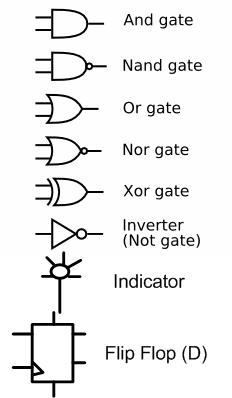
\includegraphics[scale=0.5]{images/logicSet.jpg}}
			\hfill
			\subfigure[The Electrical Symbols Dataset(EL-DS)]
			 {\label{fig:ELsymbolSet}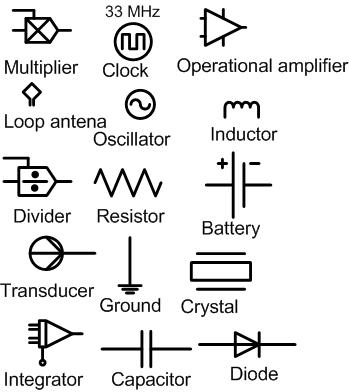
\includegraphics[scale=0.45]{images/EelectImage.jpg}}

	\caption{The datasets that were manually collected}  a)  The (LD-DS) dataset consist of symbols that are visually similar (i.e. has low shape diversity). b) The (EL-DS) dataset consist of complex topological symbols.
\end{figure}
 \begin{figure}\centering
			%\subfigure[The Digital Design Symbols Dataset(LD-DS)]{

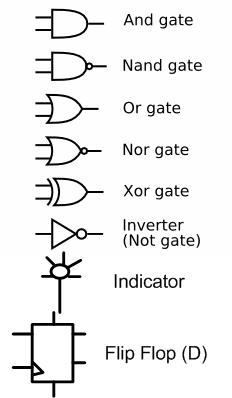
\includegraphics[scale=0.5]{images/logicSet.jpg}\label{fig:LogicsymbolSet}%}
	\caption{The Digital Design Symbols Dataset(LD-DS)}    The (LD-DS)
dataset consist of symbols that are visually similar (i.e. has low shape
diversity).
\end{figure}
\subsection{Segmentation Algorithms comparisons}
\label{sec:AlgExp}
We performed several experiments to evaluate the presented recognition system. Firstly, we tested recognition accuracy of shapes in the data set with both algorithms (\textsl{AlgS1} and \textsl{AlgS2}). We also implemented the segmentation algorithm described in \cite{earlyprocess} (\textsl{Alg3}) to compare it with our swarm algorithms. Figure \ref{fig:test1} and \ref{fig:testLD} show the accuracy achieved by each algorithm. The two swarm algorithms were tested with and without the ellipse fitting module. Combining the ellipse detection module improves the performance in certain datasets. The result shows that (\textsl{AlgS2}) gives better performance than Alg3 and AlgS1 in all datasets.  The results also shows that combining (\textsl{AlgS1} and \textsl{AlgS2} using minimum error) outperforms AlgS2 in Hs-Ds only. This behavior is explained by noticing that features are computed based on the chosen segmentation. This means that different segmentation for a symbol generates a different set of features used for recognition. This behavior affects Ls-Ds and EL-Ds more than Hs-Ds due to the higher topological and structure nature of the symbols in both datasets than of Hs-Ds.

 \begin{figure}
	\centering
	\subfigure[Algorithm comparison on HS-DS]{\label{fig:test1} 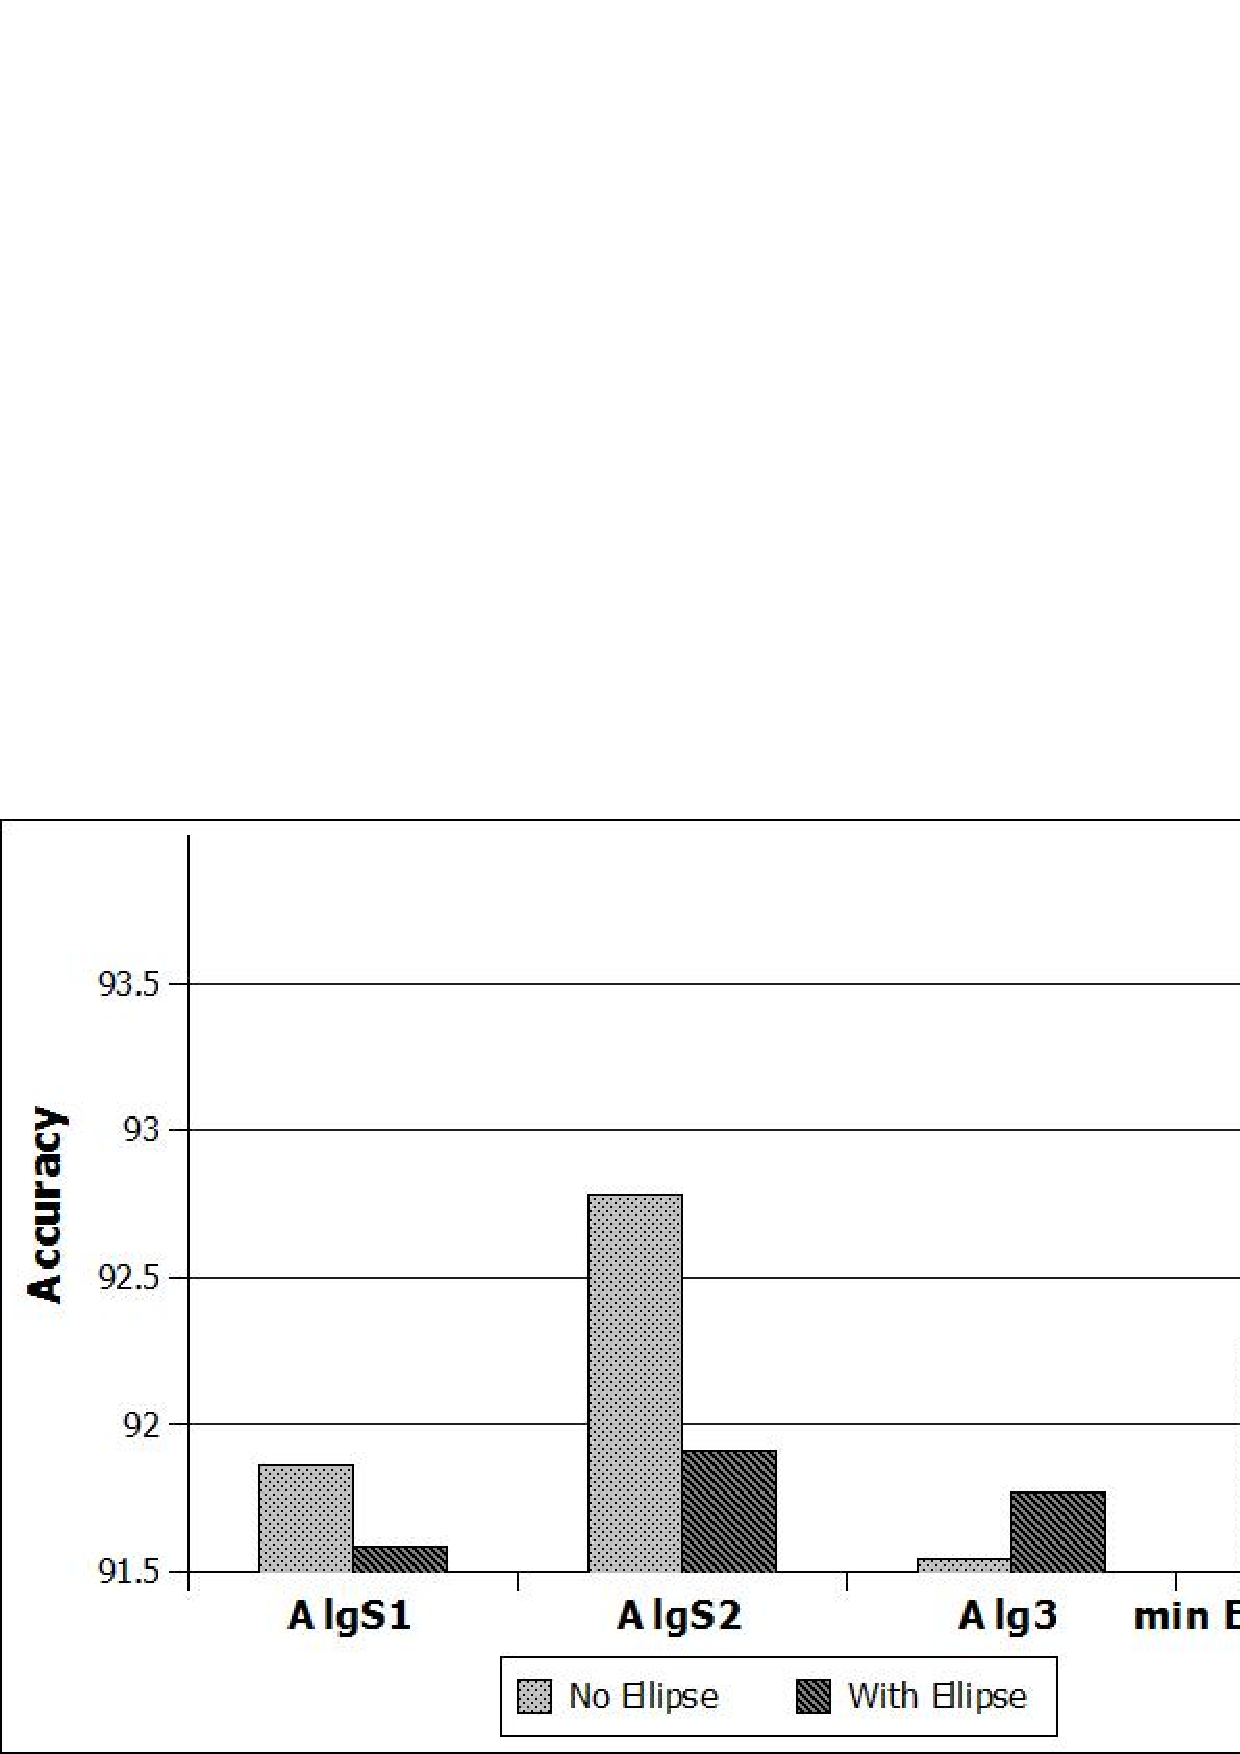
\includegraphics[scale=0.4]{images/testAlg.jpg}}
 		\subfigure[Algorithm comparison on LD-DS]{ 	 	\label{fig:testLD} 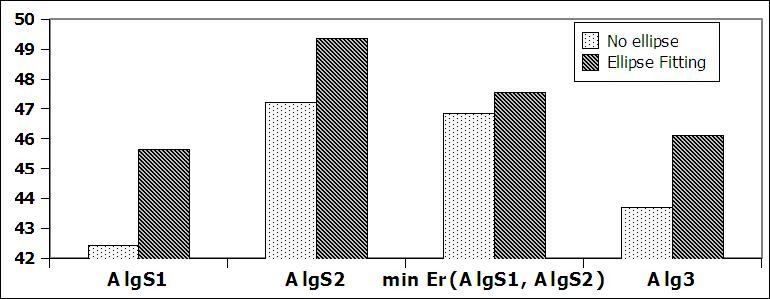
\includegraphics[scale=0.4]{images/LDAlg.jpg}}
 		\subfigure[Algorithm comparison on EL-DS]{	 	\label{fig:testEL}  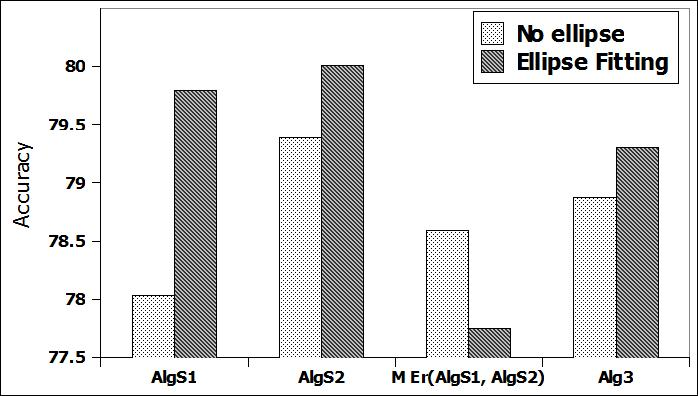
\includegraphics[scale=0.4]{images/AlgEL.jpg}}
	 	\caption{ The recognition rate of different algorithms. }
 \end{figure} 
 \subsection{Swarm Algorithms Experiments}

 Another set of tests were performed on the system to enhance non-ellipse fitting algorithms. The effect of the number of particles, the error thresholds and various other parameters were investigated. The results of these tests are shown in Figures \ref{fig:swarmtesting} and   \ref{fig:swarmtesting2}. Figure \ref{fig:swarmtesting} shows that as the number of swarm iterations increase the error value decrease (error of the segmentation algorithm). The final number of particles and maximum swarm iterations used in the system was based on a tradeoff between error achieved versus the computation time. The effect of other algorithm parameters such as $c_1$, $\omega$ (mentioned in Section\ref{sec:ParticleSwarmAlgorithm}) is tested using similar tests (Figure \ref{fig:swarmtesting2},\ref{fig:swarmwtest}).%, $c_2$

 \begin{figure}
	\centering
	 	\subfigure[Segmentation Error Vs. Swarm Iterations]{
\label{fig:swarmtesting}
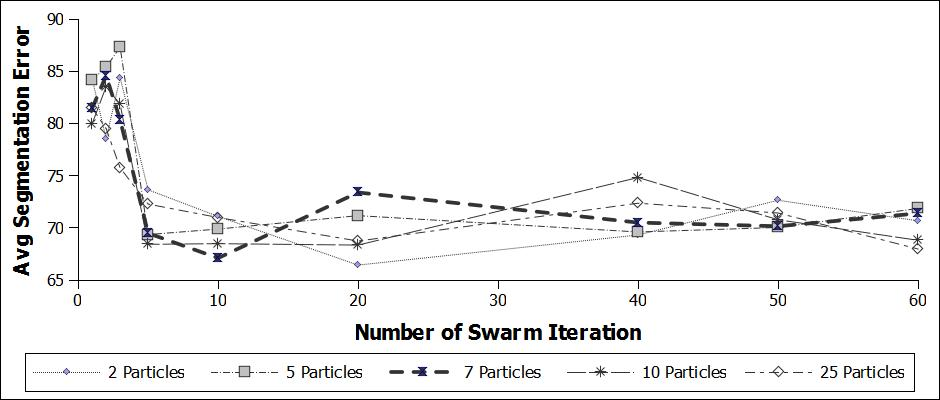
\includegraphics[scale=0.3]{images/swarmIterationVsParticles.jpg}}

		\subfigure[Segmentation Error Vs. $c_1$]{
\label{fig:swarmtesting2}  \includegraphics[scale=0.3]{images/C1Swarm.jpg}}
%swarmParamterC.jpg

				\subfigure[Segmentation Error Vs.
$\omega$]{\label{fig:swarmwtest}
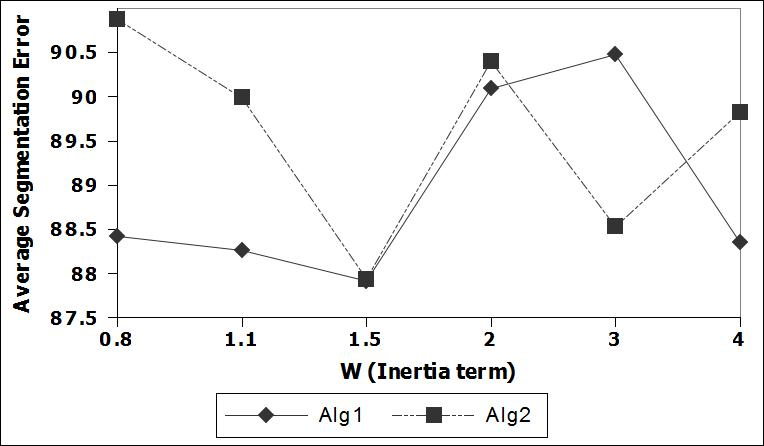
\includegraphics[scale=0.3]{images/wSwarm.jpg}} %swarmParamterC.jpg



	 	\caption{Segmentation Error Vs. PSO parameters.}a) The error
decrease as the number of swarm iteration increase until it reach a saturation.
 b) The behavior of segmentation error versus $c_1$. c) The behavior of
segmentation error versus  $\omega$.


\end{figure}

%In our experiment we used the same benchmark dataset used in \cite{mypaper},
%the dataset was collected by Hse and Newton\cite{HeloiseBeautification}. The
%data are drawn by 16 users each of them was asked to draw 13 shapes from 30 to
%50 times. Figure \ref{fig:symbolSet} shows a set of the shapes used in the data
%set. Five different splits were generated to divide the dataset into training
%and test sets. The results displayed are the average recognition accuracy of the
%five splits. The accuracy is computed as the number of correctly recognized
%samples divided by the total number of samples in the test.

%  \begin{figure}
%   \centering
%
% 		\includegraphics[scale=0.5]{symbolSet.PNG}
% 		\caption[The Symbol Set] {The symbol set}
%\label{fig:symbolSet}
% 	 \end{figure}

To demonstrate the change in accuracy is due to the enhanced swarm optimization algorithm we tested the recognition system using two sets of features. Firstly, we tested recognition accuracy of shapes in the data set with both algorithms (\textsl{AlgS1} and \textsl{AlgS2}) using the whole feature set. The second experiment was tested on both algorithms but only using half the feature set. Both experiments were compared with the Tradional PSO sketch recognition system presented in \cite{mypaper}.

Figures \ref{exp2} and \ref{exp1} show the recognition rate of each algorithm using the full feature set and half the features set respectively. The figures compares between the result that can be obtained using Traditional PSO and modifying the system using Enhanced PSO. The results show that the enhanced swarm optimization algorithm improves the segmentation of the system which leads to an increase in the recognition rate of the whole system by an average of $1.5\%$.  The increase in recognition rate is consistent in all swarm algorithms and in both experiments.
    \begin{figure}
  \centering
  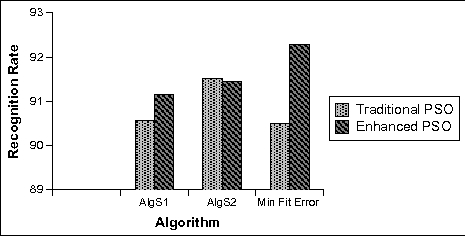
\includegraphics[width=3.3in]{Experiment_92.jpg}
  \caption[Recognition accuracy]%
  {The chart compares between recognition rate of the full feature set on both
The traditional PSO system and the Enhanced PSO. The results show that Enhanced PSO increases the performance over the  Traditional PSO. }
   \label{exp2}
\end{figure}
\begin{figure}
  \centering
  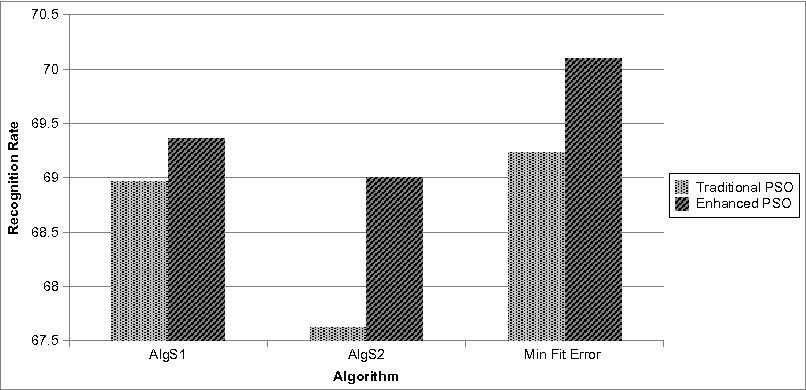
\includegraphics[width=3.3in]{Experiment_68.jpg}
  \caption[Recognition accuracy]%
  {The chart compares between recognition rate of half the feature set on both
the traditional PSO system and Enhanced PSO. The esults show that Enhanced PSO increases the recognition rate. }
   \label{exp1}
\end{figure}



\section{Conclusion }
 \label{ConclusionandFutureWork}


This paper used an Enhanced-PSO to modify a new sketch recognition using DPSO represented in \cite{mypaper}. Results show that enhancing the solutions that the \textit{PSO} in general generates an optimized stroke segmentation which improves the final recognition rate.  The final recognition improved by modifying the particle optimization algorithm without depending on the higher level features. The experiments evaluated two \textit{DPSO} different segmentation algorithms (AlgS1 and AlgS2) on simple presentation set dataset. Results show that the enhanced PSO algorithm improves the segmentation on both algorithms which achieves better segmentation and final accuracy. The results proved that the Enhancement made on the PSO improves the efficiency of the Traditional PSO algorithm without being dependable on special objective function or application. The system achieved an average overall improvement of more than 1\% over Basic PSO.

 This paper presented a new approach to sketch recognition using DPSO. The system uses multiple preliminary information, i.e., speed and curvature information, as input to the \textit{DPSO}. Results show that the \textit{DPSO} in general generates an optimized stroke segmentation which improves the final recognition rate.  The final recognition is based on both global shape and hierarchical stroke properties. Adding stroke and segment geometrical features improved the final recognition. Global shape and moment properties were used to prevent the need to use graph matching which is computationally expensive \cite{SketchRead2007}. The experiments evaluated two \textit{DPSO} different segmentation algorithms (AlgS1 and AlgS2) on three different datasets (Hs-Ds, EL-Ds and LD-Ds). Results show that AlgS2 achieves better segmentation and final accuracy than Alg3 \cite{earlyprocess} on the datasets used. The results proved that the system is easily expandable to more and more symbols as it does not depend on low level primitive recognizers but on high level symbol and geometrical features.  The system achieved an average overall improvement of more than 2\% over Alg3 in all datasets.

   The tradeoff between accuracy achieved and time complexity can be further investigated to achieve better results. Currently, the system processes one symbol at a time, an enhancement would be to allow users to draw more than one symbol at a time and incorporate a method for separating symbols. Thus, possible extension of this research is to complete the clustering algorithm for fully automated sketch recognition. Another area of enhancements is the features extraction methods. Introducing more spatial and geometrical features is believed to improve classifications. Features that represent the appearance of the symbols are likely to improve the recognition of symbols that have similar geometrical structure (i.e. Nor and OR gate in logic symbols).
 

 For the future work, it is suggested that we continue to improve both the enhanced PSO segmentation algorithm. Also, a possible extension of this research is to improve the recognition algorithm of the Sketch Recognition system. Other area of enhancements is the features extraction methods. Introducing more spatial and geometrical features is believed to improve classifications.

%\bibliographystyle{natbib}
\bibliographystyle{ieeetr}
\bibliography{../../../neededfiles/Bibliographies/Mybibliography}

\end{document}


